\begin{figure}
    \centering
    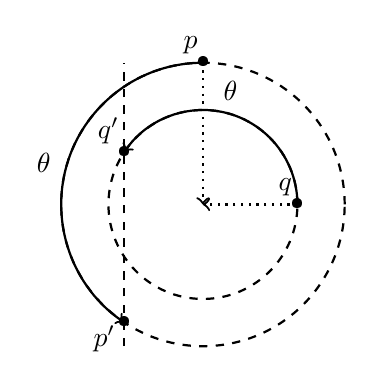
\begin{tikzpicture}[thick, scale=0.6]
        \node[label={[label distance = -3mm]160:$p$}] at
            (0, 3) {\textbullet};
        \node[label={[label distance = -3mm]160:$q$}] at
            (2, 0) {\textbullet};

        \draw[->, dotted] (0, 3) -- (0, 0); % p arrow
        \draw[->, dotted] (2, 0) -- (0, 0); % q arrow

        \draw[dashed] (0,0) circle[radius=3];
        \draw[dashed] (0,0) circle[radius=2];

        \draw[->] (0, 3) arc(90:236:3) node[midway, xshift=-3mm] {$\theta$};
        \draw[->] (2, 0) arc(0:146:2) node[midway, yshift=3mm] {$\theta$};
        \node[label={[label distance = -3mm]160:$q'$}] at
            (-1.6634, 1.1104) {\textbullet};
        \node[label={[label distance = -3mm]260:$p'$}] at
            (-1.6634, -2.4952) {\textbullet};

        \draw[dashed] (-1.664, -3) -- (-1.664, 3); % p arrow
    \end{tikzpicture}
    \caption{Exemplo de parâmetro de evento horizontal ocorrendo
    entre $p$ e $q$, com a trajetória simulada.}
    \label{degen:exemploeventos}
\end{figure}